\chapter{Smart Grid Power Flow Status Monitoring}



\section{Smart grid Monitoring}
The \acrlong{sg} system constitutes a complex system of subsystems, which proper operation is a prerequisite for the successful transmission of electric energy from producers to consumers. 
In order for the \acrshort{wams} to receive status monitoring data, a controlled process for retrieving, transmitting, and more often than not temporarily storing, sensor data is a prerequisite for proper system operation.



\subsection{Description of the Smart Grid  Monitoring system}
Electricity is produced according to the current demand for energy, as controlled by the Demand Management system, dynamically adjusting the energy supply accordingly. In order to successfully reply to the dynamically changing demands for energy, a close monitoring of the production, transmission and distribution of energy is required. In order for the monitoring system to obtain status information, the proper transmission of monitoring data from power status sensors to the   \acrshort{wams}  is essential.


\section{Storing and transmitting data for monitoring}


\subsection{Introduction}




\subsection{Phasor Measurene units}


\begin{figure}%[ht]
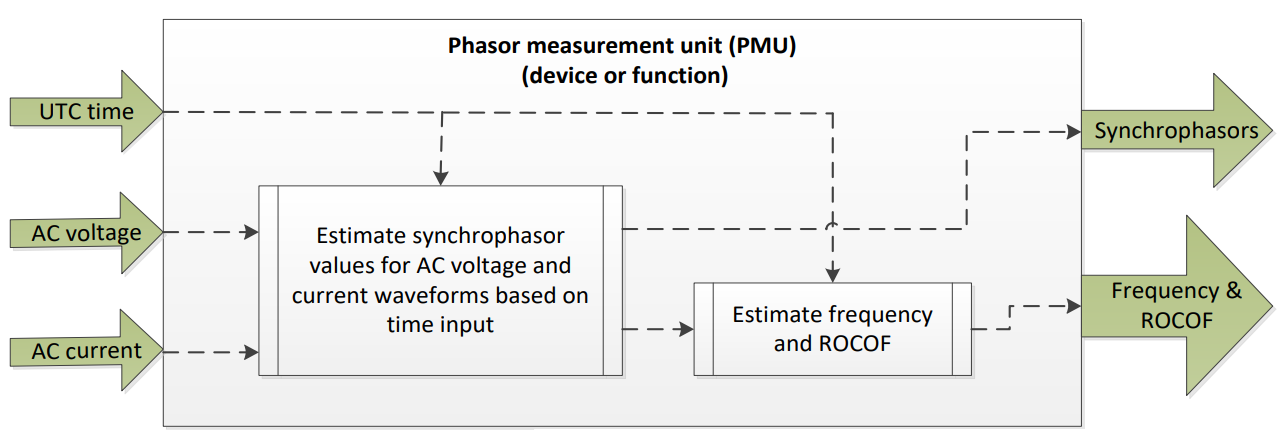
\includegraphics[width=\linewidth]{figures/PMU-in-out.png}
\caption[PMU inputs and outputs]{PMU inputs and outputs, as presented in \Cite[p.12]{iec2018measuring}
}
\label{fig:PMU-in-out}
\end{figure}

\subsection{Phasor data Concentrator}




\subsection{Time Synchronisation Protocols}

\section{Introduction}
Time Synchronisation protocols are used in order to synchronise the time of interconnected devices in need of synchronised time for various purposes. In the case of synchrophasor devices, the devices needs to be time synchronised in order for \acrshort{sg} \acrshort{wams} operators to get a correct overview of the system state.



The \acrshort{ptp} is included in the IEC standard

%\subsection{Synchrophasor data alignment attack}
Eq \ref{DMS} about DMS, and  eq \ref{DSM} about DSM.






\subsection{Synchrophasor Protocols}
\cite[p. 11]{johnson2018standards} figure 2

The introduction of Synchrophasors in the \acrlong{pg}, 

\subsubsection{Introduction}



As described in \cite{martin2011synchrophasor} and \cite{ali2016performance}, the \acrfull{pmu}, along with the \acrfull{pdc}, were introduced in the 1980s. The communication and data exchange from the PMU to the PDC was standardised by the introduction of the IEEE 1344 standard in 1995, which was the standard communication protocol for synchrophasor data exchange, until the introduction of the IEEE C37.118 in 2005.
The  IEEE C37.118 protocol was derived from the original IEEE 1344 standard, and has undergone a number of revisions, over the years.


In \cite{martin2013synchrophasor}, \citeauthor{martin2013synchrophasor}describes the history of ...

\begin{itemize}
    \item The IEEE C37.118-2005,
    \item The IEEE C37.118-2011
    \item The IEEE C37.118-2018
\end{itemize}




%Unlike the \acrlong{cpg}, the \acrlong{sg} enables bidirectional flow of power, by customers operating micro grids enabling customers to sell excessive power back to the network.








%\section{Historical}
%SCADA monitoring flaws -> PMU




%\section{PMUs}
%PMU
%-  Descripton of PMU
%- phasor
%- synchronised phasors
%- Communication with PDC

%\section{PDCs}
%PDC
%- Collecting synchronised phasors from PMU
%- Grouping synchronised phasors with same timestamp into Synchrophasor record
%- At deadline, transmitting Synchronaised phasors, received before deadline.
%- Improved security. 
%\section{Synchrophasors}
%Synchrophasors
%- overview
%- sync precision requirements:
 
%\section{Protocols used for monitoring}
%Protocols
%- Figure from PowerPoint
%- Concentrating on upper left side of figure.


%- capabilities of x.2011 x=synchrophasor protocol

%PTP
%Rationale for concentrating on PTP
%Descriptino of the protocol
%Time synchronisation via PTP
%PTP delay attack (types)


\section{Time Synchronisation}
In order to synchronise the samples received from the \acrshort{pmu}, the \acrshort{pdc}, as well as the \acrshort{pmu} devices producing the samples, is required to adjust their clock by utilising a precise and reliable times source.  Given the distributed nature of the \acrshort{pmu} devices providing samples from locations distributed over a Wide Area Network, the \acrfull{gps} is the  time source selected. 

\subsection{Introduction}


The dependency on networking favors the usage of low-cost \acrshort{gnss} receivers for synchronising time between the growing number of \acrshort{pmu}s deployed at various locations, monitoring energy flow states of the highly distributed \acrshort{sg}. 



\subsubsection{The Importance of Time Synchronisation}

In \cite{dagle2019importance}, \citeauthor{dagle2019importance} states the following aspects as the benefits for Smart Grid operation, of ensuring correct time synchronisation:


\begin{itemize}
    \item  Situational Awareness and Wide-Area Monitoring
    \item  Real-Time Operations
    \item  Power System Planning 
    \item  Forensic Event Analysis
    
\end{itemize}

\subsubsection{Possible effects of Time Synchronisation errors}
Timing errors will, according to ,,, render the data introduced to the \acrshort{wams} system inadequate to enable \acrshort{sg} operatiors to get overview of the Energy supply state of the \acrshort{sg}.

In \Cite{martin2019impact}, \citeauthor{martin2019impact} lists a number of side-effects which could result form the absence of high-quality data material from the \acrshort{wams}.


\begin{enumerate}




    \item Data loss,
    \item Data corruption,
    \item Inaccurate representation of engineering quantities,
    \item Lack of precision,
    \item Incorrect measurement identification,
    \item Excessive or inconsistent latency.

\end{enumerate}

\subsubsection{Precision Time Protocol services}
The \acrfull{ptp} is a network-based time protocol, enabling the time difference between devices to be synchronised within a fraction (in the order of a few $\mu$s) of a second, satisfying the requirements of the \acrshort{sg}. 

\begin{figure}[ht]
    \centering
    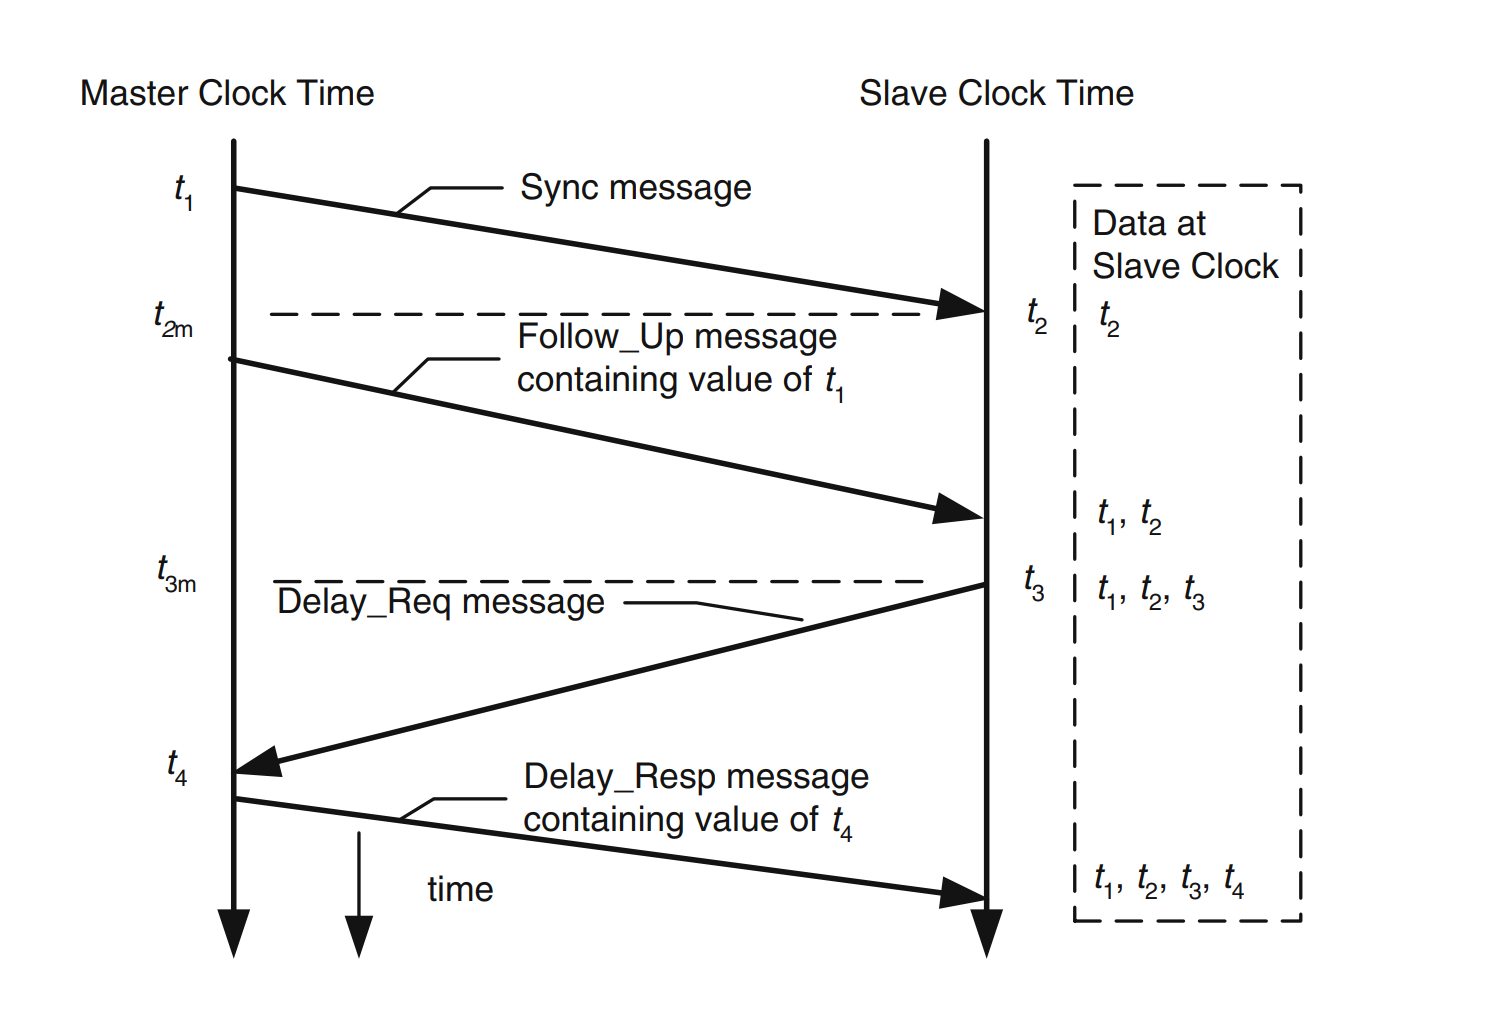
\includegraphics[ width=\textwidth]{figures/PTP-timing-Diagram.png}
    \caption[Timing diagram for synchronization messages]{As presented in \cite[p. 51]{Eidson2006}: Timing diagram for synchronization messages.} 
    \label{fig:PTP-timing-Diagram}
\end{figure}  

\subsubsection{Description of PTP time synchronisation}



A device, being synchronised  by the \acrshort{ptp} protocol, reads its system time from a slave clock, being periodically synchronised with a master clock.


The time of the slave clock, is being adjusted according to the following process:


Following the message exchange visualised by \figureautorefname { } \ref{fig:PTP-timing-Diagram}, the Slave clock  uses the time offset from the Master clock time, $offset = [(t_2 - t_1) + (t_4 - t_3)]\div 2$, in order to synchronise with the Master clock. 
In order to be able to achieve the time difference required, the \acrshort{ptp}, as described by  \citeauthor{Eidson2006}, in \cite{Eidson2006}, is dependant on:

\begin{itemize}
    \item Timestamped network events, messages, which is  used for synchronisation.
    \item A method of timestamp transmission as required for synchronisation.
    \item Overcoming any timing impairments introduced by system components.
\end{itemize}




\subsection{Smart Grid Time Synchronisation}



\subsubsection{Introduction}


The \acrlong{sg} is dependant on precise Time Synchronisation, as a Time Synchronisation error of a few $\mu$-seconds may result in \acrshort{sg} instability. The time stamps produced by Synchrophasors, pinpointing the exact time of any system event, is vital in order to ensure precise and reliable system state information.
In the event of a system alert being triggered by erroneous system state Information, corrective actions by operators might have undesired effects. 

\subsubsection[Smart Grid Time Sync Precision Requirements]{Smart Grid Time Synchronisation Precision Requirements}

In order to ensure the time precision required for the \acrshort{sg}, the correct selection of time synchronisation mechanisms is vital. 




\begin{figure}%[ht]
    \centering
    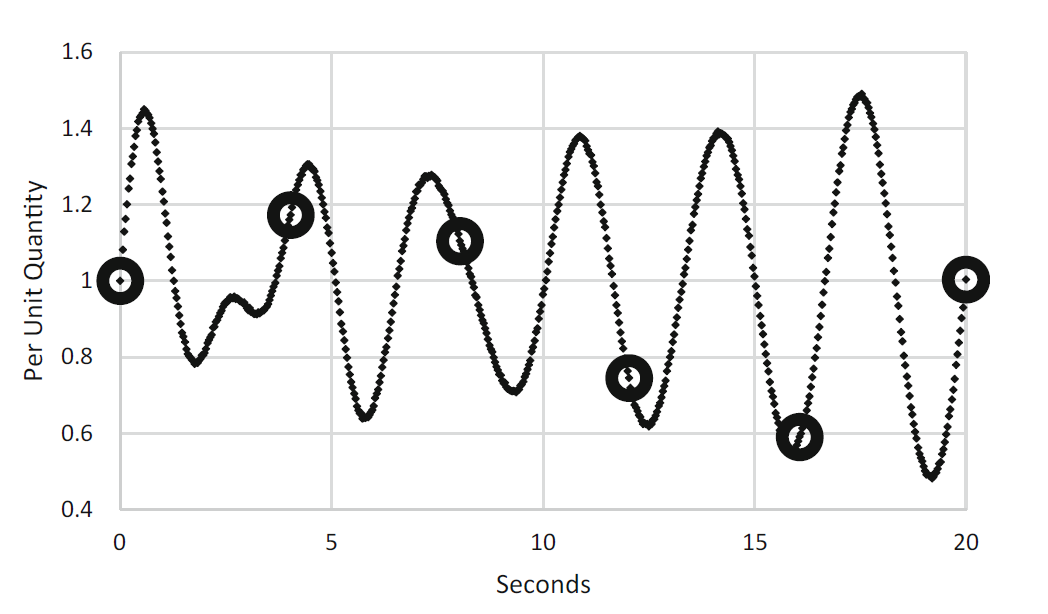
\includegraphics[ width=\textwidth]{figures/syncrophasors-vs-scada.png}
    \caption[Difference between Synchrophasor and SCADA measurements]{As presented in \cite[p. 3]{dagle2019importance}: Notional representation of the difference between synchrophasor and SCADA
measurement. Figure credit: \citeauthor{dagle2019importance}}.
    \label{fig:syncrophasors-vs-scada}
\end{figure}  

\subsection{Synchrophasor}
%\cite{ali2016wide}


%\Cite{rana2015exploring}



The \acrshort{pmu} is receiving values from sensors, on which it is able to calculate voltage level and phase angle of the energy flow. It is utilising a time-source to pinpoint measurements in time, producing synchrophasors, to be transmitted to the nearest \acrshort{pdc}. 

As described by \citeauthor{dagle2019importance} in \cite{dagle2019importance}, the data received from traditional \acrshort{scada} systems are time-stamped after arriving at the control station. The synchrophasors of the \acrshort{wams} on the other hand are, as described by \Citeauthor{ali2016wide} in \cite{ali2016wide}, being time-stamped in real-time before being transferred to the control system. The sampling rate of the \acrshort{pmu}, results in synchrophasor data enabling operators of the \acrshort{wams} to get real-time visualisation of critical elements, like the state of energy flow  of the \acrlong{sg}. The increased granularity of the measurement system allows for the detection of anomalies undetectable by traditional \acrshort{scada} systems, as illustrated by \figureautorefname { }\ref{fig:syncrophasors-vs-scada}. 

The increased sampling rate, of the synchrophasors of the \acrshort{wams} systems enables a more fine-grained view of energy distribution system state changes. However, in order for the \acrshort{wams} system to get the correct system state information, correct time stamps is critical. 
Therefore, the time-synchronisation mechanisms of the \acrshort{pmu} system is of critical importance. \\ 

\begin{figure}
    \centering
    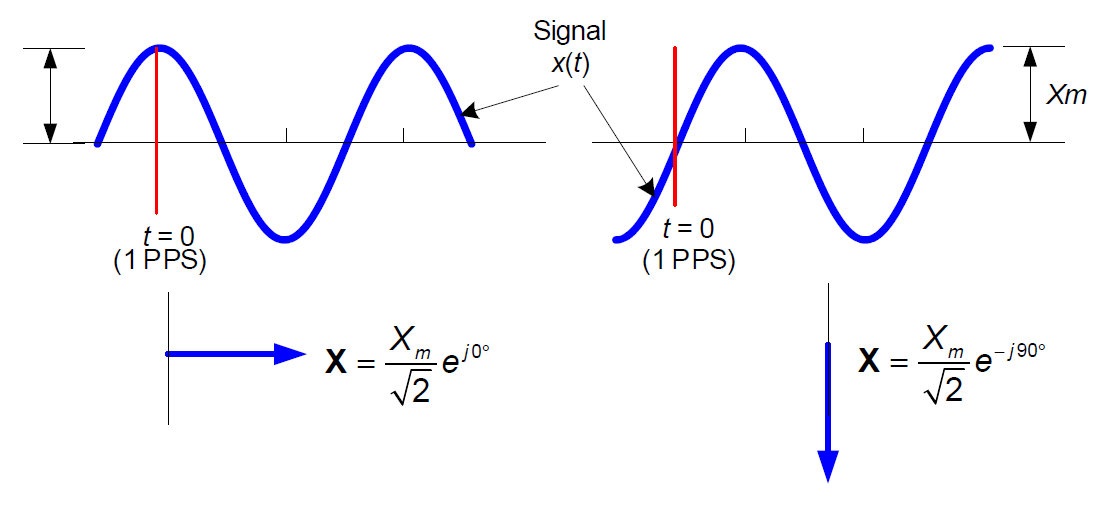
\includegraphics[ width=\textwidth]{figures/Synchrophasor-Definition.png}
    \caption[Convention for synchrophasor representation]{As presented in \Cite{schofield2018design}: Convention for synchrophasor representation.}.
    \label{fig:Synchrophasor-Definition}
\end{figure}  
